\documentclass{article}
\usepackage{polski}
\usepackage[utf8]{inputenc}
\usepackage[version=3]{mhchem} % Package for chemical equation typesetting
\usepackage{siunitx} % Provides the \SI{}{} and \si{} command for typesetting SI units
\usepackage{graphicx} % Required for the inclusion of images
\usepackage{natbib} % Required to change bibliography style to APA
\usepackage{amsmath} % Required for some math elements 

\setlength\parindent{0pt} % Removes all indentation from paragraphs

\renewcommand{\labelenumi}{\alph{enumi}.} % Make numbering in the enumerate environment by letter rather than number (e.g. section 6)

%\usepackage{times} % Uncomment to use the Times New Roman font

%----------------------------------------------------------------------------------------
%	DOCUMENT INFORMATION
%----------------------------------------------------------------------------------------

\title{Michał Bronikowski\protect \\ \hfill \newline \newline Systemy Operacyjne 2017\\ Problem złodzieja jabłek\\ } % Title

%\author{Michał \textsc{Bronikowski}} % Author name

\date{\today} % Date for the report

\begin{document}

\maketitle  % Insert the title, author and date
\newpage
\tableofcontents
\newpage
%----------------------------------------------------------------------------------------
%	OPIS 1
%----------------------------------------------------------------------------------------

\section{Opis zadania}

\subsection{Problem złodzieja jabłek}
Problem został przeze mnie wymyślony na potrzeby zadania. Wzorowałem sie na klasycznym problemie synchronizacji tj. problemie producenta i konsumenta. Powiedzmy, że jesteśmy złodziejem jabłek i w naszej miejscowości są dwa sady A i B, w których w dość szybkim tępie przybywa jabłek. Kradniemy jabłḱa z sadu A lub z sadu B. W międzyczasie w sadach, dzięki działaniu właścicieli i natury jabłek przybywa. Problem polega na takim zsynchronizowaniu procesów sadów A i B oraz procesu złodzieja, żeby złodziej nie ukradł wszystkich jabłek z sadów, ponieważ to zwróciłoby uwagę właściciela i nasz złodziej mógłby mieć problemy.
\subsection{Rozwiązanie}
Rozwiązanie składa się z trzech procesów. Procesu złodzieja i dwóch procesów reprezentujących sady. 
Do synchronizacji procesów użyję semaforów. W celu zabezpieczenia dostępu do sekcjii krytycznych programu użyję Mutex'ów.
%----------------------------------------------------------------------------------------
%	OPIS 2
%----------------------------------------------------------------------------------------

\section{Opis implementacji}
Program skłąda się z jednego pliku źródłowego \textbf{sem.c}.\\ W programie możemy wyróżnić następującą strukturę:
\begin{center}
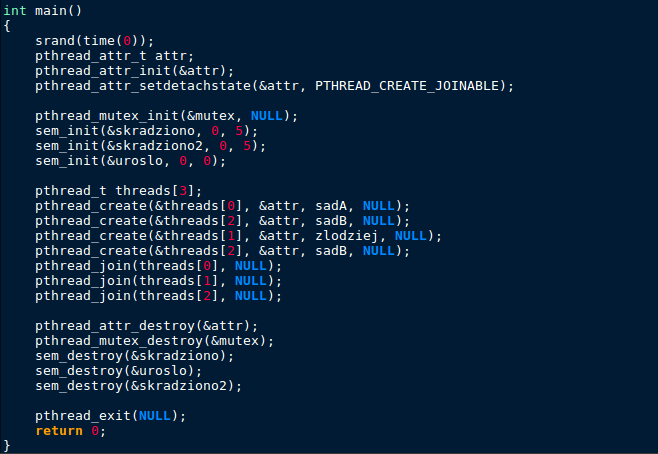
\includegraphics[width=\textwidth]{main} 
\caption{Funkcja głowna programu}
\end{center}

\begin{center}
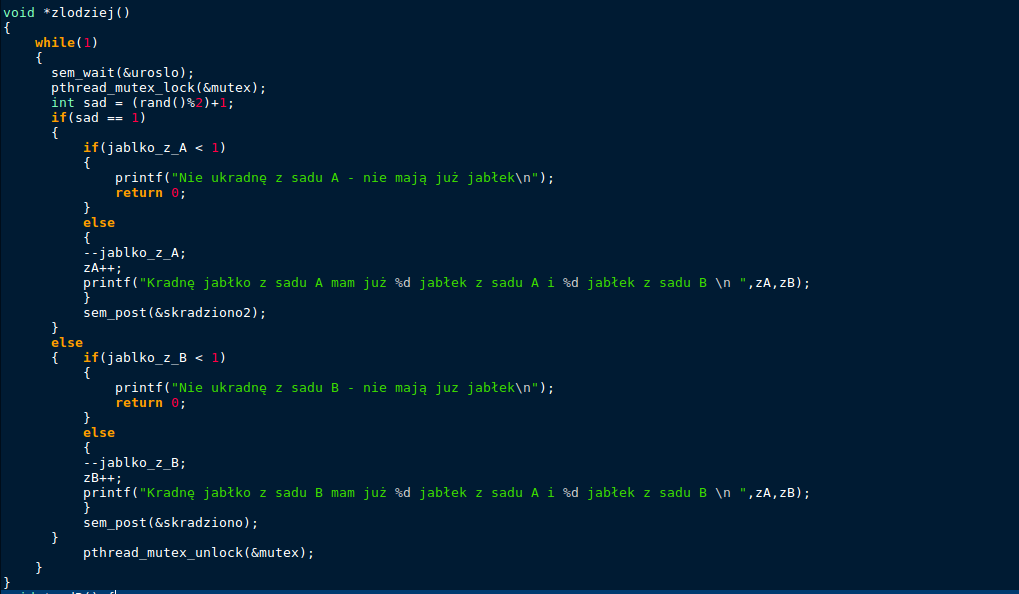
\includegraphics[width=\textwidth]{zlodziej} 
\caption{Funkcja zarządzająca procesem złodzieja}
\end{center}

\begin{center}
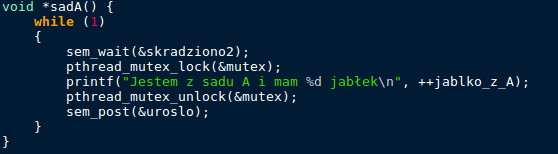
\includegraphics[width=\textwidth]{sadA} 
\caption{Funkcja zarządzająca procesem sadu A}
\end{center}

\begin{center}
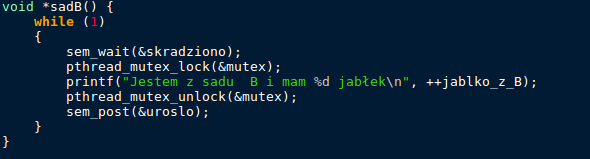
\includegraphics[width=\textwidth]{sadB} 
\caption{Funkcja zarządzająca procesem sadu B}
\end{center}

Na początku inicjalizuję semafory o nazwach:\textbf{ skradziono,uroslo,skradziono2 }. Inicjalizuję również mutex dający dostęp do zasobów  tylko jednemu wątkowi. Następnie tworzę 3 wątki: \textbf{sadA,sadB,zlodziej}. Procesy odpowiadające za ,,produkcję" jabłek w sadach są zwalnianie przez semafory \textbf{skradziono} i \textbf{skradziono2}. Każdy z procesów sadów informuje o tym, że zwiększyła się ilość dostępnych jabłek. Proces złodzieja losowo wybiera, z którego sadu chce ukraść jabłka, jeżeli w danym sadzie nie ma już jabłek oznacza to, że synchronizacja nie działa poprawnie i wtedy program kończy swoje działanie. Każdorazowo po kradzieży złodziej zwalnia odpowiedni semafor prrzypisany do sadu A lub sadu B. Na starcie w każdym sadzie jest dziesięć jabłek oraz wartości odpowiadających im semaforom ustawione są na pięć, a złodzieja na zero. Taki zabieg pozwala nam uniknąć sytuacji w której złodziej będzie chciał ukraść jabłka z sadu, w którym tych jabłek nie ma.

\section{Testowanie}
Program należy uruchamiać na systemie operacyjnym LINUX. Do kompilacji służy komenda: \\
\textbf{gcc -pthread -o sem sem.c  } \\ 
\begin{center}
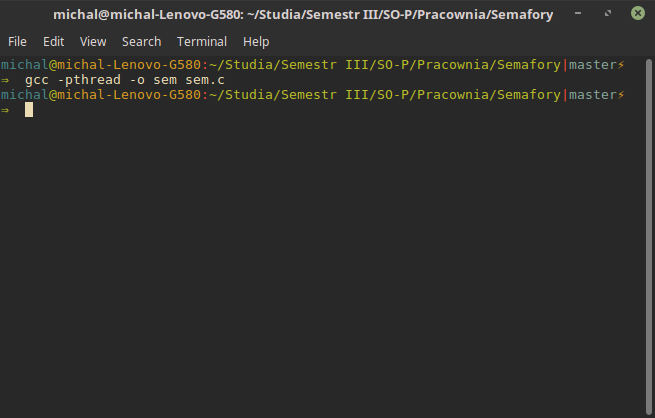
\includegraphics[width=\textwidth]{kompilacja} 
\caption{Kompilacja}
\end{center}
Wersja binarna programu będzie dostępna pod nazwą \textbf{sem}, uruchamiamy poleceniem: \\
\textbf{./sem}
\begin{center}
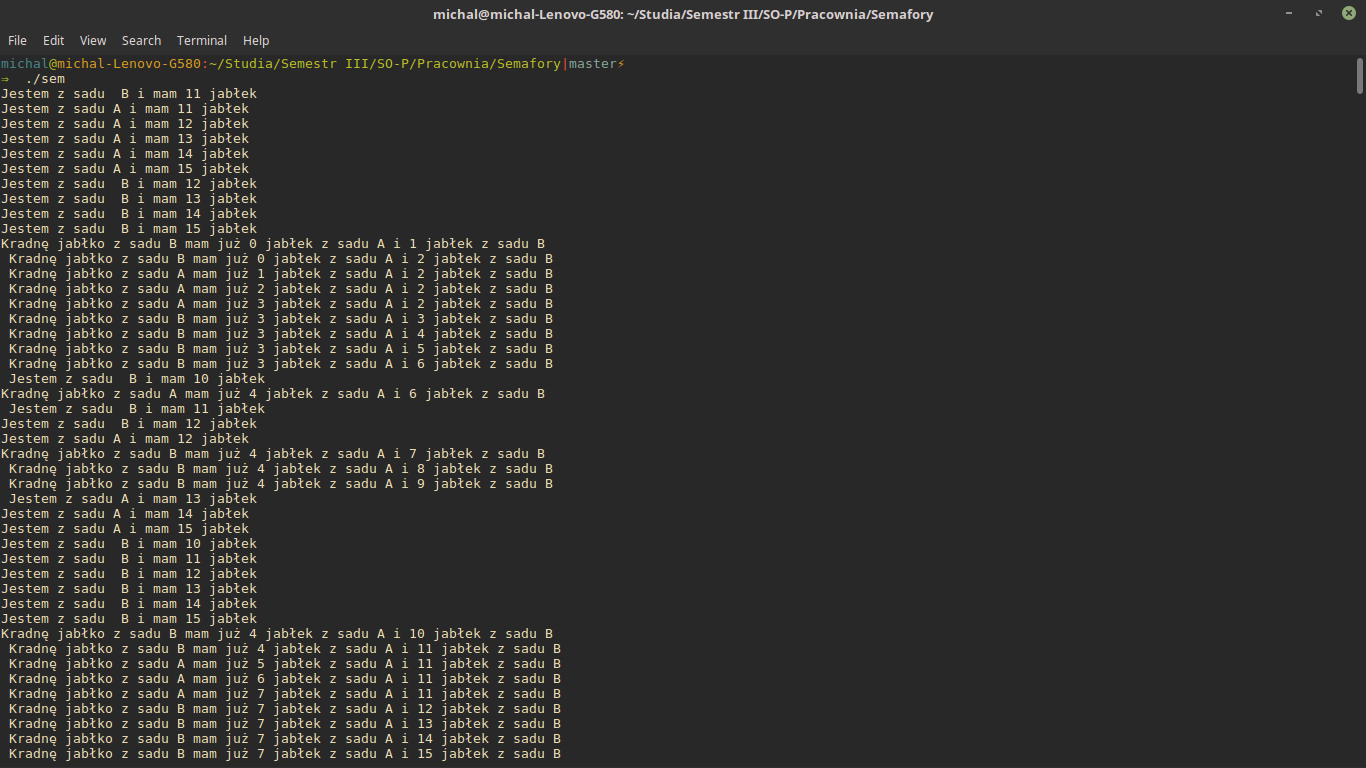
\includegraphics[width=\textwidth]{uruchomienie} 
\caption{Uruchomienie}
\end{center}
Program powinien działać poprawnie ze względu na wartości startowe semaforów odpowiadających za sady. Tyle jeżeli chodzi o teorię, wykonałem jeszcze test, polegający na tym że uruchomiłem ten program w tle i przez 5h się nie zatrzymał.
\end{document}